El sistema debe adaptarse al sistema operativo Linux. Anticipado a futuros cambios en la plataforma se decide trabajar con Node.js, ya que es de código abierto y multiplataforma, esto permite beneficiarse de la reutilización del código y la falta de cambio de contexto. Las aplicaciones Node.js están escritas en JavaScript puro y pueden ejecutarse dentro del entorno Node.js en Windows, Linux, etc.
\vspace{0.8cm}

La interfaz gráfica de usuario de la aplicación debe ser responsiva y funcionar en la mayoría de los navegadores web modernos, además debe ser fácil de aprender, idealmente requerir poco entrenamiento.
\vspace{0.8cm}

\subsection{Herramientas}
Node.js permite incorporar herramientas poderosas a proyectos de cualquier tipo. Esto incluye todo, desde bibliotecas y \glspl{framework} como jQuery y AngularJS hasta procesadores de código como Webpack. Los paquetes vendrán en una carpeta típicamente llamada node\_modules, que también contendrá un archivo package.json. Este archivo contiene información sobre todos los paquetes, incluidas las dependencias, que son módulos adicionales necesarios para usar un paquete en particular.

\subsubsection{Dependencias de desarrollo}
Las dependencias de desarrollo son aquellas que se utilizan dentro del entorno de programación. Aquí se incluyen herramientas que no forman parte del ejecutable final como lo son lo preprocesadores, empaquetadores y analistas de código. Los principales módulos de desarrollo son los siguientes:
\begin{itemize}
  \item Babel: es un compilador de JavaScript utilizado para convertir código ECMAScript 2015+ (ES6+) en una versión que pueda ser ejecutado en motores JavaScript más antiguos.
  \item Webpack: es un empaquetador de módulos principalmente para JavaScript, pero puede transformar archivos \gls{frontend} como HTML, CSS e imágenes si se incluyen los complementos correspondientes.
  \item ESLint: es una herramienta de análisis de código estático para identificar patrones problemáticos encontrados en el código JavaScript.
  \item PostCSS: es una herramienta de desarrollo de software que utiliza complementos basados en JavaScript para automatizar las operaciones de rutina de CSS. Con este modulo es posible analizar CSS, agregar prefijos de proveedor a las reglas CSS, ejecutar optimizaciones enfocadas, para garantizar que el resultado final sea lo más pequeño posible para un entorno de producción.
  \item Pug: es un preprocesador que simplifica la tarea de escribir HTML. También agrega funcionalidades, como objetos Javascript, condiciones, bucles, \glspl{mixin} y plantillas.
\end{itemize}

\subsubsection{Estructura del proyecto}
La estructura del proyecto Node.js está influenciada por preferencias personales, la arquitectura del proyecto y la estrategia de inyección de módulos que se está utilizando. Para tener una estructura FERN, es imperativo separar el código fuente del servidor y el utilizado por el cliente, ya que el código del lado del cliente o \gls{frontend} probablemente se minimizará y se enviará al navegador y es público en su naturaleza básica. Y el lado del servidor o el \gls{backend} proporcionarán \acrshort{api} para realizar operaciones \acrshort{crud}.

\subsubsection{Directorios}
\begin{itemize}
  \item node\_modules: Directorio oculto que contiene las dependencias generales del proyecto, este archivo debe ser ignorado por el controlador de versiones.
  \item server: Aquí se encuentran los archivos requeridos por el servidor para el enrutamiento, la conexión con la base de datos y las funciones de utilidad del \gls{backend}.
  \item src: Este directorio concentra todos los elementos necesarios para producir nuestra aplicación cliente.
  \item views: En esta carpeta se incluyen los templates necesarios para generar las vistas HTML de nuestro proyecto.
  \item www: Su propósito es contener los archivos del cliente, aquí podemos encontrar el código de producción de nuestra aplicación web compilado y minificado, así como las hojas de estilo, imágenes, fuentes tipográficas, vectores, etc.
\end{itemize}

\subsubsection{Archivos principales}
\begin{itemize}
  \item .babelrc: Contiene los mecanismos necesarios para compilar sintaxis moderna de JavaScript y una lista con los navegadores web a los que se requiere dar enfoque.
  \item .env: Documento oculto que contiene las variables del entorno, este archivo es ignorado por el controlador de versiones.
  \item .eslintrc.js: En este archivo se declaran las reglas para identificar e informar sobre patrones o errores encontrados en el código.
  \item .gitignore: Aquí se describen los archivos y directorios que deben ser ignorados por Git.
  \item index.js: Entrada principal de nuestro servidor, contiene el código necesario para que el proyecto funcione correctamente.
  \item package.json: Este archivo puede contener muchos metadatos sobre su proyecto. Pero principalmente se usa para dos cosas:
  \begin{itemize}
    \item Gestionar dependencias de su proyecto
    \item Scripts, que ayudan a generar compilaciones, ejecutar pruebas y otras cosas con respecto al proyecto
  \end{itemize}
\end{itemize}

\begin{figure}[H]
  \centering
  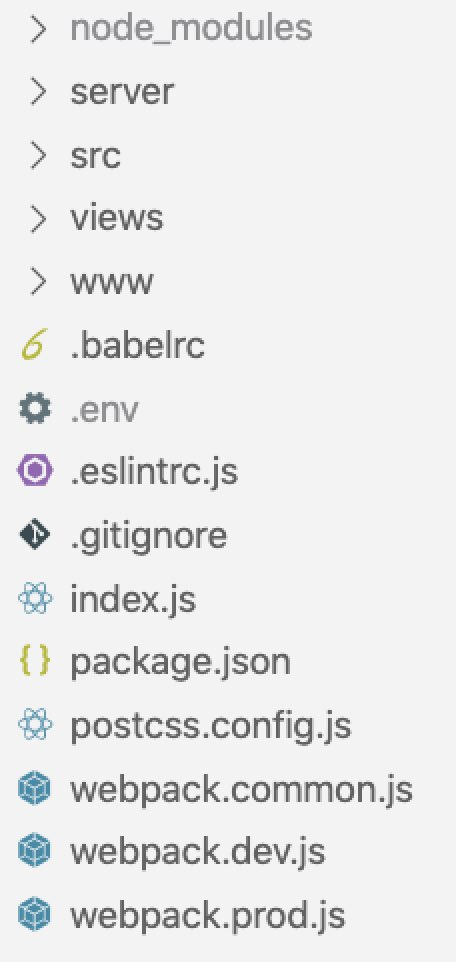
\includegraphics[width=0.3\textwidth]{app}
  \caption{Vista general de la raíz del proyecto. (Fuente: Elaboración propia)}
\end{figure}

\newpage
\subsubsection{Variables del entorno}
El acceso a las variables de entorno en Node.js es compatible desde el primer momento. Cuando el proceso Node.js se inicia, automáticamente proporciona acceso a todas las variables de entorno existentes al crear un objeto env como propiedad del objeto global del proceso.
\vspace{0.8cm}

\lstinputlisting[style=ES6, caption=Variables principales del sistema]{code/env.txt}
